% Choose the report format
\documentclass[11pt]{article}
\usepackage[
    a4paper,
    left=20mm,
    right=20mm,
    top=20mm,
    bottom=20mm
    ]{geometry}
\renewcommand{\baselinestretch}{2}
\usepackage{setspace} % set 1.5 spacing
\onehalfspacing
\usepackage{helvet} % set font type
\renewcommand{\familydefault}{\sfdefault}
\usepackage{fancyhdr}

% Encoding parameters (always necessary ?)
\usepackage[utf8]{inputenc}
\usepackage[T1]{fontenc}
\usepackage[french]{babel}

% Make some reference, bibliography and others
\usepackage{biblatex}
\addbibresource{biblio.bib}

\usepackage{wrapfig}
\usepackage{hyperref}
\usepackage{caption}

% For the math symbol in latex equations
\usepackage{amsmath}

% For 
\usepackage{graphicx}
\graphicspath{{../fig/} }

\begin{document}
    
    %-------------------------
    % Page de Garde
    %-------------------------

    \pagestyle{fancy}
    \fancyfoot{}
    \fancyfoot[L]{Aix-Marseille Université}
    \fancyfoot[R]{2023/2024}
    \vspace{5cm}

    \begin{center}
        \Large \textbf{Analyse du report des voix entre les deux tours des élections législatives anticipées de 2024.}
    \end{center}
    
    \vspace{2cm}
    
    \begin{center}
        Mémoire en vu de l'obtention du Diplôme d'Etudes Supérieures Universitaires de Data Science \\
        \textit{par Alexandre Lainé}
    \end{center}

    \newpage
    % Document format
    \pagestyle{fancy}
    \fancyhead{} % clear all header fields
    \fancyhead[L]{Alexandre Lainé}
    \fancyhead[R]{Mémoire DESU de Data Science}
    \fancyfoot{} % clear all footer fields
    \fancyfoot[R]{\thepage}

    %-------------------------
    % Intro, Question Scientifique et Contexte (1page)
    %-------------------------
    \section{Introduction}

    Peu après les élections européennes de 2024, durant lesquelles la liste du Rassemblement National (RN), portée par Jordan Bardella et Marine Le Pen, a obtenu 37 \% des suffrages \cite{Le_Monde_2024a}, le Président de la République a décidé de dissoudre l'Assemblée nationale et de déclencher des élections législatives anticipées. Après un premier tour record pour le RN, c'est finalement le Nouveau Front Populaire (NFP ou Union de la Gauche, UG) qui est arrivé en tête (182 sièges) après un entre-deux-tours rythmé par les désistements et les consignes de vote visant à faire barrage au RN dans un maximum de circonscriptions \cite{Wikipédia_2024a}.

    \begin{wrapfigure}{R}{0.4\textwidth}
        \begin{center}
            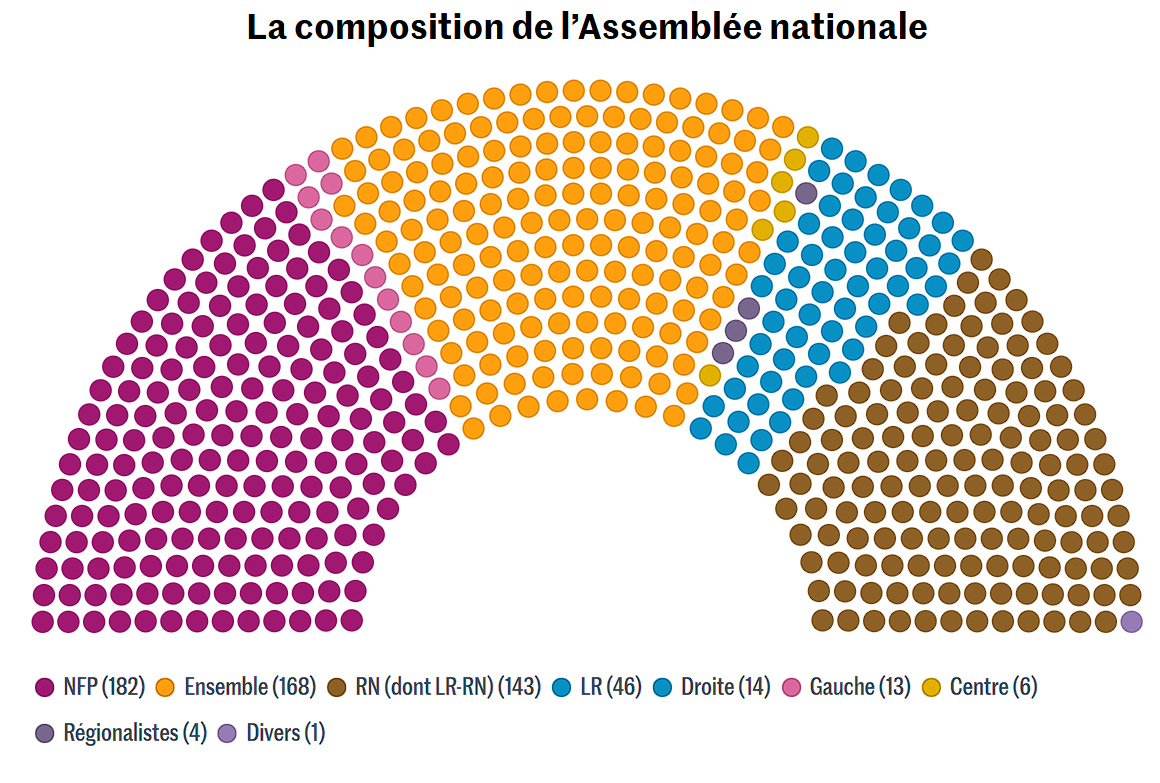
\includegraphics[width=0.38\textwidth]{Resultats_2024.png}    
        \end{center}
        \caption{Répartition de l'assemblée nationale suite aux élections législatives anticipées de 2024 \cite{Le_Monde_2024b}.}
    \end{wrapfigure}

    Ces mouvements de voix sont particulièrement intéressants, et il est possible de se demander si les résultats du premier tour sont suffisants pour prédire le déroulement du second. Basé sur cette interrogation, il s'agit donc de trouver une règle décrivant les mouvements de voix entre les deux tours. Depuis la publication des résultats, très peu de travaux ont été publiés. La seule approche utilisée à ma connaissance, et ne se basant pas sur des sondages, est celle de l'apprentissage statistique \cite{Amblard_2024}, visant à estimer le taux de report entre les "familles" politiques. Celui-ci prend alors la forme d'une distribution sur l'ensemble des circonscriptions décrite par une moyenne et une variance particulières. Néanmoins, cette approche ne répond pas tout à fait à la question posée. En guise de base à ce travail, il a déjà été décrit une approche d'apprentissage automatique permettant d'estimer le transfert des voix entre les deux tours des élections présidentielles de 2022 sous la forme d'une matrice \cite{Perrinet_2022}. Cependant, dans le cas des élections législatives, le problème est plus complexe, car dans chaque circonscription, les nuances des candidats du second tour peuvent être différentes. Cela ajoute à l'hétérogénéité des bureaux de vote une forte diversité en raison du grand nombre de face-à-face possibles.

    L'objectif de ce projet est donc d'utiliser cette approche d'apprentissage automatique afin de trouver une matrice représentant le taux de transfert de voix de chaque partie du premier tour vers celles du second tour. Il est nécessaire de passer par plusieurs niveaux de complexité : tout d'abord, en regroupant les différentes nuances politiques sous la forme de "familles", puis en restreignant l'apprentissage à des cas particuliers de face-à-face, avant de tenter la phase la plus complexe en essayant l'apprentissage sur l'ensemble des bureaux de vote. 
    
    S'agissant d'un sujet actuel, l'objectif n'est ici en aucun cas de "refaire le match" mais seulement d'utiliser des outils issus de l'intelligence artificielle afin d'analyser les données de ces élections en se concentrant sur les mouvements de voix, notamment dus à la mise en place d'un "front républicain". Ce terme, apparu pour la première fois à l'occasion des élections législatives de 1956, prend racine dans la défense républicaine qui a eu lieu au début de la Troisième République afin de faire barrage aux élans monarchistes.
    
    \newpage
    %-------------------------
    % Matériel et Méthodes (3pages)
    %-------------------------
    \section{Matériel et Méthodes}

        \subsection*{Jeux de donnés}
            Les résultats des élections législatives pour le premier et le second tour sont disponibles pour chaque bureau de vote en France métropolitaine, dans les Territoires d'Outre-Mer, ainsi qu'à l'étranger en accès libre sur le site du gouvernement \cite{République_Française}. Ces fichiers, d'environ 40 Mo pour le premier tour et 16 Mo pour le second tour, fournissent pour chaque bureau de vote le nombre de voix obtenues par candidat, ainsi que le nombre d'inscrits, le nombre d'abstentions et le nombre de bulletins nuls.
        
        \subsection*{Pré-processing des données}
            De manière générale, l'objectif de cette phase de prétraitement est de supprimer les colonnes et les lignes vides, ainsi que les informations non nécessaires pour la suite, telles que le genre, le nom et le prénom des candidats, le nom des communes et des départements. Les bureaux de vote n'ayant pas eu besoin de second tour sont également exclus, car ils ne fournissent pas d'informations sur le report des voix. Il est important de noter qu'avant toute étape d'apprentissage, le jeu de données est divisé en deux parties : la première pour l'entraînement du modèle et la seconde pour évaluer sa précision sans influencer l'apprentissage. De plus, bien que le tableau ne contienne que le nombre de voix obtenues par chaque nuance, la première étape de la fonction d'apprentissage consiste à diviser le nombre de voix obtenues par chaque nuance dans un bureau de vote par le nombre total de voix exprimées dans ce bureau de vote.

            Afin de progresser dans la complexité de la tâche d'apprentissage automatique, trois approches pour préparer le jeu de données seront différenciées :
        
            \begin{itemize}
                \item[--] Regroupement des nuances en "familles" politiques : L'objectif est de rassembler les résultats des nuances présentes dans chaque bureau de vote en grands groupes, en se basant sur leur positionnement dans le spectre politique \cite{Wikipédia_2024b}. 
                \item[--] Focalisation sur les bureaux de vote avec des face-à-face particuliers : Cette approche se concentre principalement sur les bureaux de vote ayant généré un important report de voix en raison de la présence du Rassemblement National au second tour et des désistements qui en découlent. 
                \item[--] Conservation de toute la complexité des élections : Cette méthode conserve toutes les informations, mais exclut le nombre d'abstentions, de votes nuls et de votes blancs. 
            \end{itemize}
        
            \noindent Le regroupement des nuances en "familles" est réalisé comme suit : 
            \begin{itemize} 
                \item[--] EXTGAUCHE+ : Extrême gauche, France Insoumise, Parti Communiste, Parti Radical de Gauche. 
                \item[--] GAUCHE+ : Union de la Gauche, Écologiste, Socialiste, Divers Gauche. 
                \item[--] CENTRE+ : Ensemble, Horizon, Union des Démocrates et Indépendants, Divers Centre. 
                \item[--] DROITE+ : Les Républicains, Divers Droite. 
                \item[--] DIVERS+ : Divers, Les Écologistes, Droite Souverainiste, Régionaliste. 
            \end{itemize}

        \subsection*{Modèle de transfert de voix}
            Si on considère le pourcentage de voix obtenu par chaque partie dans un bureau de vote comme une distribution discrète notée $D$, l'hypothèse est qu'il existerait une matrice de transition $M$ permettant de faire le lien entre les distributions du premier et second tour (respectivement $D_1$ et $D_2$). Mathématiquement, cela s'exprime comme suit :
            \begin{equation}
                \hat{D_2} = D_1 \times M
            \end{equation}
            L'objectif est donc d'utiliser les résultats du premier et du second tour afin d'apprendre de façon automatique cette matrice $M$ qui a $n$ lignes et $m$ colonnes, correspondant respectivement au nombre de nuances au premier et au second tour. Ce modèle de transfert de voix sera donc constituer d'une couche d'entrée dont la taille correspond au nombre de nuances politiques présentent au premier tour dans toute la France, mais aussi d'une couche de sortie, dont la taille correspond au nombre de nuances présentent au second tour (figure \ref{fig:Model}). La matrice $M$ correspond par conséquent aux poids reliant la première à la seconde couche. 
            
            \begin{figure}
                \begin{center}
                    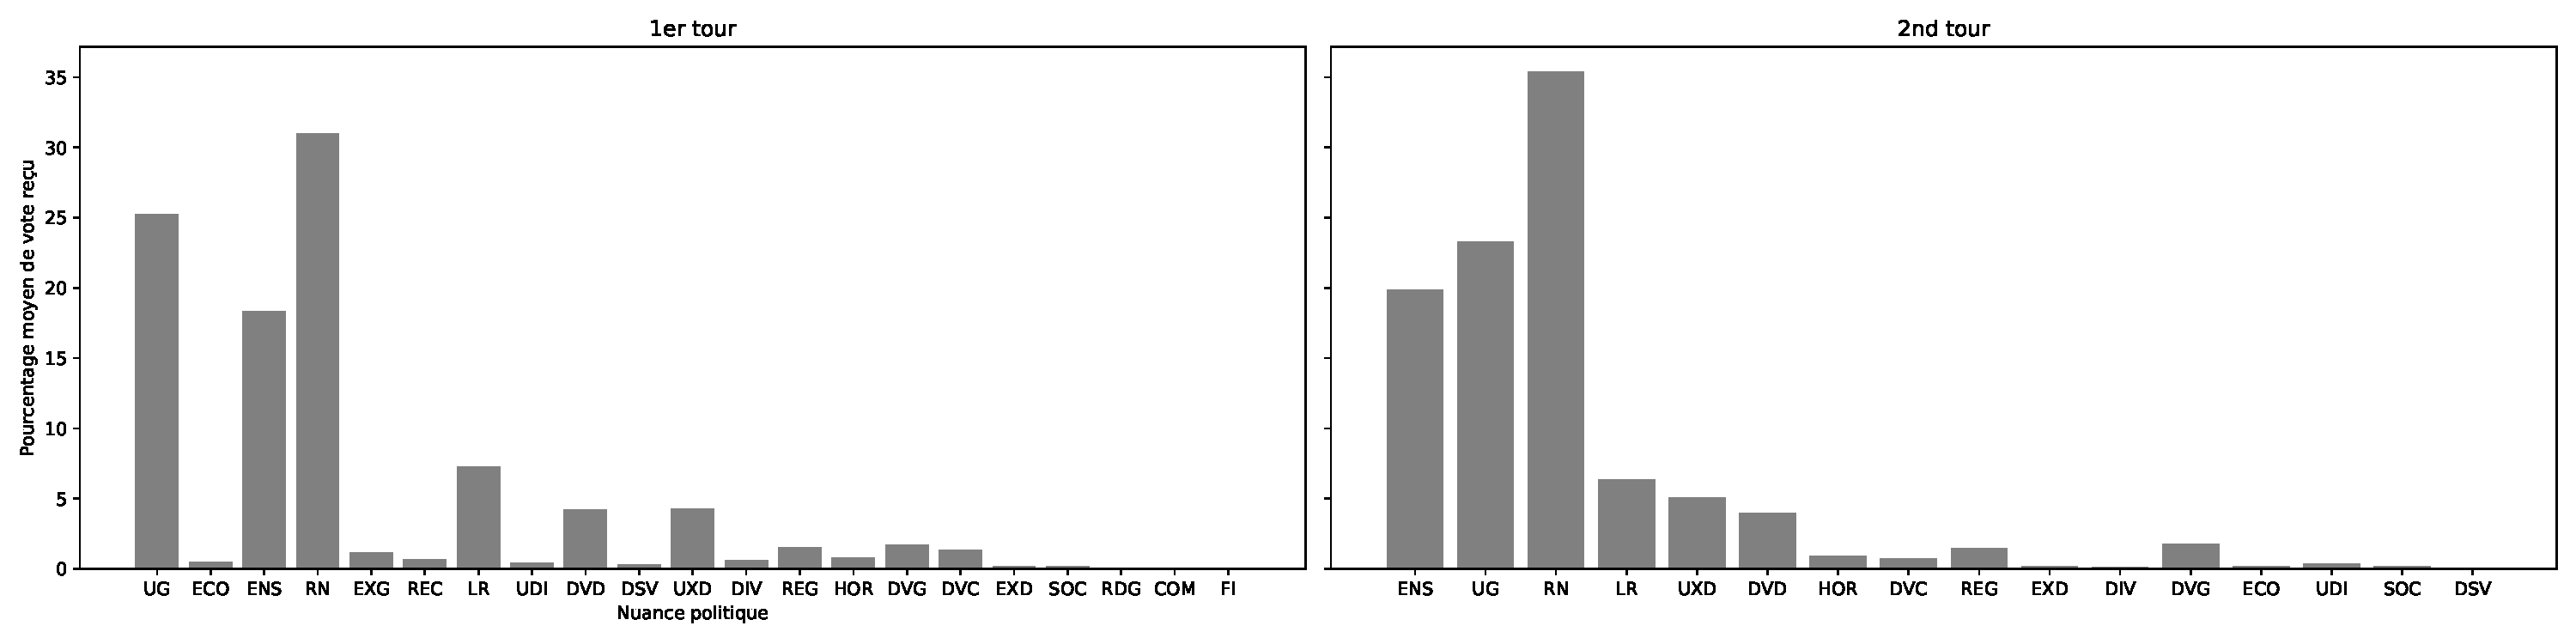
\includegraphics[height=6cm]{Distribution_votes_1er_et_2nd_tour.pdf}
                    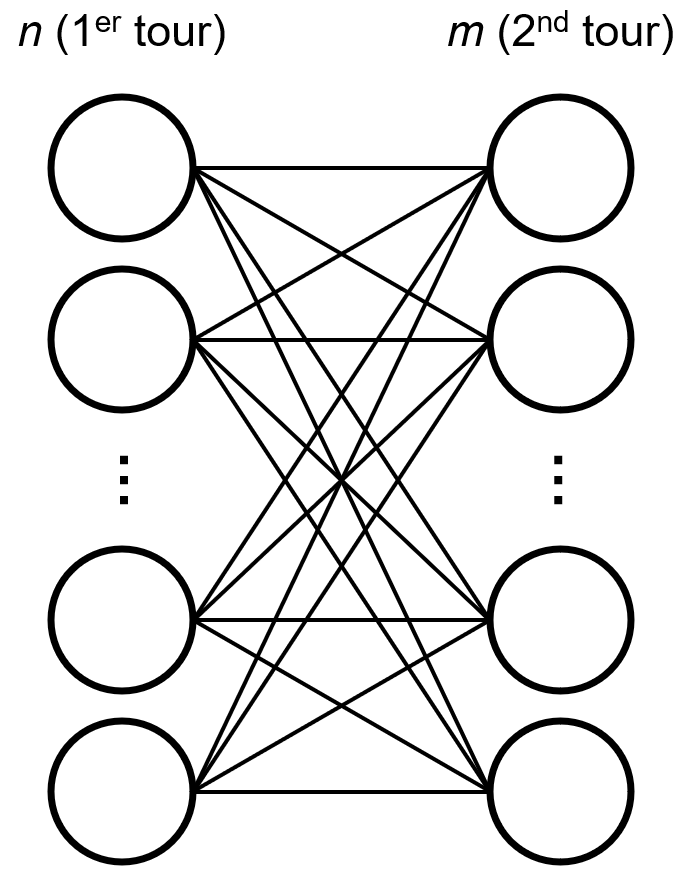
\includegraphics[height=6cm]{Model_transfert_Voix.png}
                    \caption{Gauche) Distribution moyenne des votes entre les différentes sur l'ensemble des bureaux de vote. Droite) Représentation shématique du modèle utilisé.}
                    \label{fig:Model}
                \end{center}
            \end{figure}

        \subsubsection*{Divergence de Kullback-Leilbler}
            La divergence de Kullback-Leilbler \cite{Kullback_Leibler_1951} ($KL$) est une mesure permettant la comparaison entre deux distributions de probabilités discrètres. Celle-ci nous permettra de comparer la distance entre les distributions réelles du second tour ($D_2$) et celles prédites par notre modèle ($\hat{D_2}$) selon la formule suivante :
            \begin{equation}
                KL(D_2,\hat{D_2}) = \sum_{k \in \Omega} D_2 \cdot \log \frac{D_2}{\hat{D_2}}
            \end{equation}

        \subsubsection*{Entrainement et contrôle}
            Bien qu'il soit possible d'incorporer une fonction de stop anticipé pour l'apprentissage, le choix effectué ici a été de tester différents nombres d'itérations et de stopper l'apprentissage dès que le résultat de la fonction de coût, sur la partie de validation, se stabilise. La descente de gradient est réalisée à l'aide d'une implémentation PyTorch de l'algorithme d'optimisation Adam, qui est particulièrement efficace pour les jeux de données volumineux et pour l'optimisation d'un grand nombre de paramètres \cite{Kingma_Ba_2017}.

        \subsection*{Visualisation et représentations graphiques}
            Afin de visualiser le jeu de données et de rendre compte des différents résultats obtenus dans cette pipeline, il a été choisi d'utiliser principalement les bibliothèques matplotlib (version 3.9.0) et seaborn (version 0.13.2) pour leur simplicité d'utilisation, ainsi que plotly (version 5.24.0) pour la qualité de ses graphiques interactifs et sa capacité à gérer une grande quantité de données. La plupart des figures créées dans la pipeline sont automatiquement enregistrées au format PDF dans le dossier "fig" de la pipeline.
            
        \subsection*{Information supplémentaires}
            L'ensemble du code de la pipeline est disponible en libre accès sur la plateforme GitHub en cliquant simplement \href{https://github.com/alexandre-laine/Pipeline_Elections_Legislatives}{ici}. Toute l'analyse a été développée et écrite pour le mémoire du DESU en utilisant le langage de programmation Python (version 3.11.9) ainsi que la librairie open source PyTorch \cite{Ansel_Yang_He_Gimelshein_Jain_Voznesensky_Bao_Bell_Berard_Burovski_et_al._2024}, principalement sous la forme de notebooks appelant des fonctions écrites par mes soins. Les calculs ont été réalisés en local sur mon ordinateur personnel (OMEN by HP Laptop 16-xf0xx) avec les caractéristiques suivantes : CPU : AMD Ryzen 9 7940HS, GPU-1 : AMD Radeon 780M, GPU-2 : NVIDIA GeForce RTX 4070.

    \newpage
    %-------------------------
    % Résultats (4pages)
    %-------------------------
    \section{Résultats}
        
        \subsection*{Grandes "familles" politiques}
            
        Cette première partie vise à répondre de manière simplifiée à la question en considérant uniquement de grandes "familles" politiques. Il a été possible d'estimer la matrice de transition entre les deux tours, comme illustré sur la partie gauche de la figure \ref{fig:Famille}. On y observe qu'un groupe au premier tour influence majoritairement son propre groupe au second tour. Sur la partie centrale de la figure \ref{fig:Famille}, les pourcentages prédits dans chaque bureau de vote sont comparés aux pourcentages réels pour évaluer la précision de la prédiction. Bien que certains points se situent correctement sur la diagonale rouge, on peut distinguer deux groupes de points qui s'écartent de cette diagonale : certains présentent une surévaluation du nombre de voix, tandis que d'autres montrent une sous-évaluation.
            
            \begin{figure}[h]
                \begin{center}
                    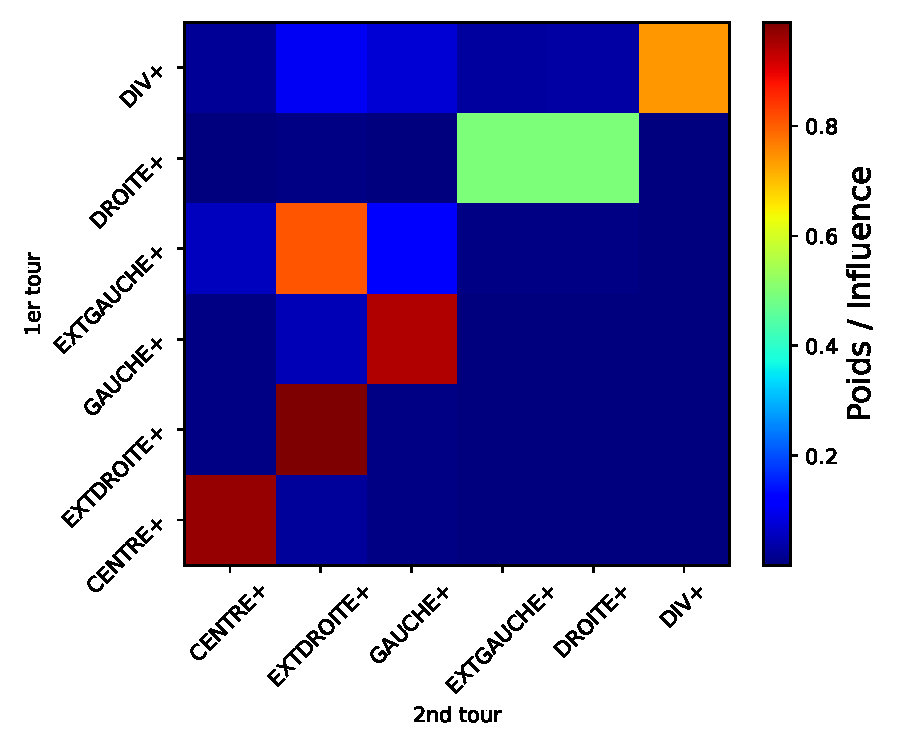
\includegraphics[height=4cm]{Famille_Matrice.pdf}
                    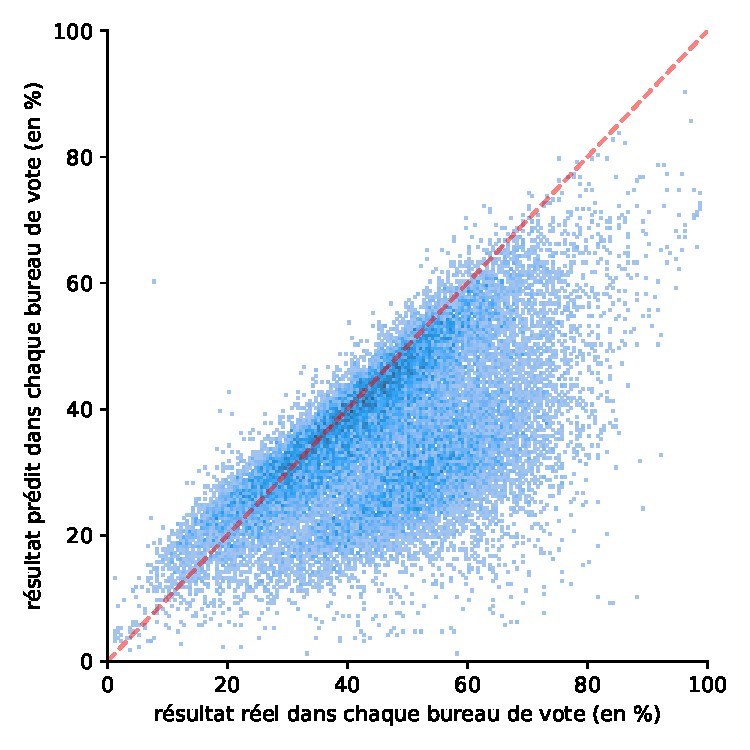
\includegraphics[height=4cm]{Famille_True_Pred_Hist.pdf}
                    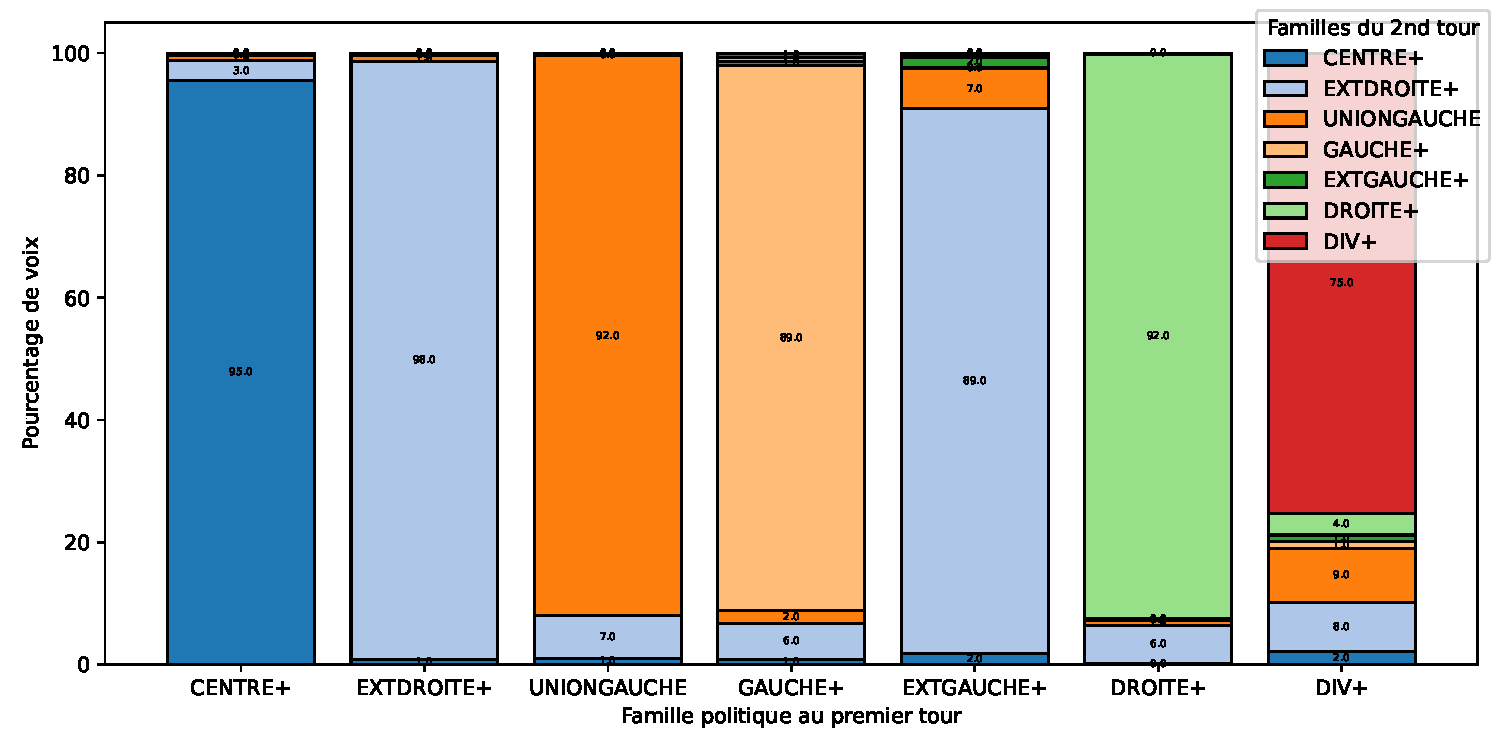
\includegraphics[height=4cm]{Famille_Proportions.pdf}
                    \caption{Gauche) Matrice de transition de l'entre deux tour estimée. Centre) Comparaison entre les valeurs prédites et réelle par le biai un d'un histogramme en deux dimensions. Droite) Représentation estimée de chaque "familles" du premier tour dans les résultats des "familles" du second tour.}
                    \label{fig:Famille}
                \end{center}
            \end{figure}

        \subsection*{Face-à-face}

            Afin de complexifier la tâche, nous pouvons nous concentrer uniquement sur les bureaux de vote présentant des face-à-face pour étudier le report des voix de manière plus spécifique. Le premier élément confirmant que l'apprentissage de la matrice de transition s'est bien déroulé est résumé dans la figure \ref{fig:Focus_pred_true}. Contrairement à la figure précédente, nous ne remarquons cette fois-ci aucun autre groupe que celui situé sur la diagonale.
            
            Cette seconde partie aurait donc mieux fonctionné. En vérification post-analyse, il est possible de représenter le pourcentage de report de chaque partie du premier tour en fonction de la nuance du candidat présent au second tour. On observe alors des mouvements qui semblent logiques, tels que le report des voix de l'Union de la Gauche évitant systématiquement le Rassemblement National (voir figures \ref{fig:ENS-RN} et \ref{fig:LR-RN}), avec 90 \% et 85 \% de report respectivement vers Ensemble et les Républicains. De la même manière, mais dans une moindre mesure, Ensemble présente un report de 70 \% vers l'Union de la Gauche et de 80 \% vers les Républicains (voir figures \ref{fig:LR-RN} et \ref{fig:UG-RN}). Pour les nuances rares, les pourcentages de report sont plutôt équivalents, probablement en raison du faible nombre d'exemples, sauf dans le cas de fortes affinités politiques (DVG et EXG vers UG, REC vers RN).

            \begin{figure}
                \begin{center}
                    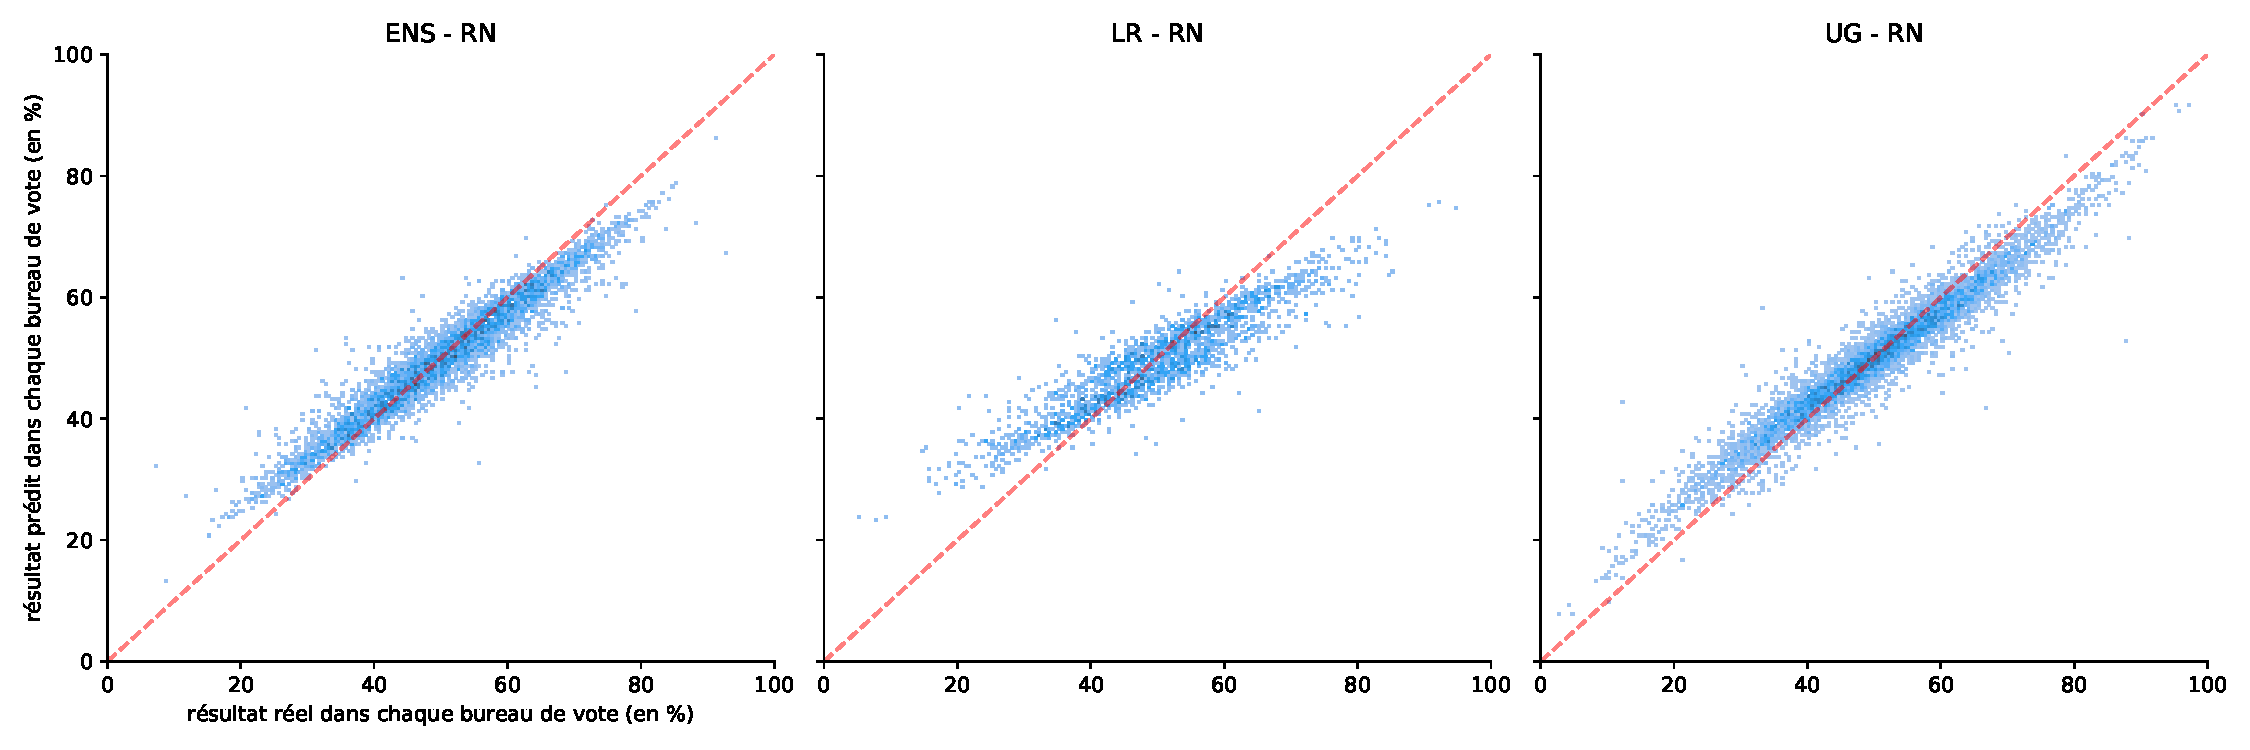
\includegraphics[width=0.9\textwidth]{Focus_True_Pred_Hist.pdf}
                    \caption{Histograme bi-dimensionnel de chaque type de face-à-face du score prédit en fonction du score réel. Créé avec des fenêtres 1 \% la couleur indique la densité de point dans la zone.}
                    \label{fig:Focus_pred_true}
                \end{center}
            \end{figure}
            
            \begin{figure}
                \begin{center}
                    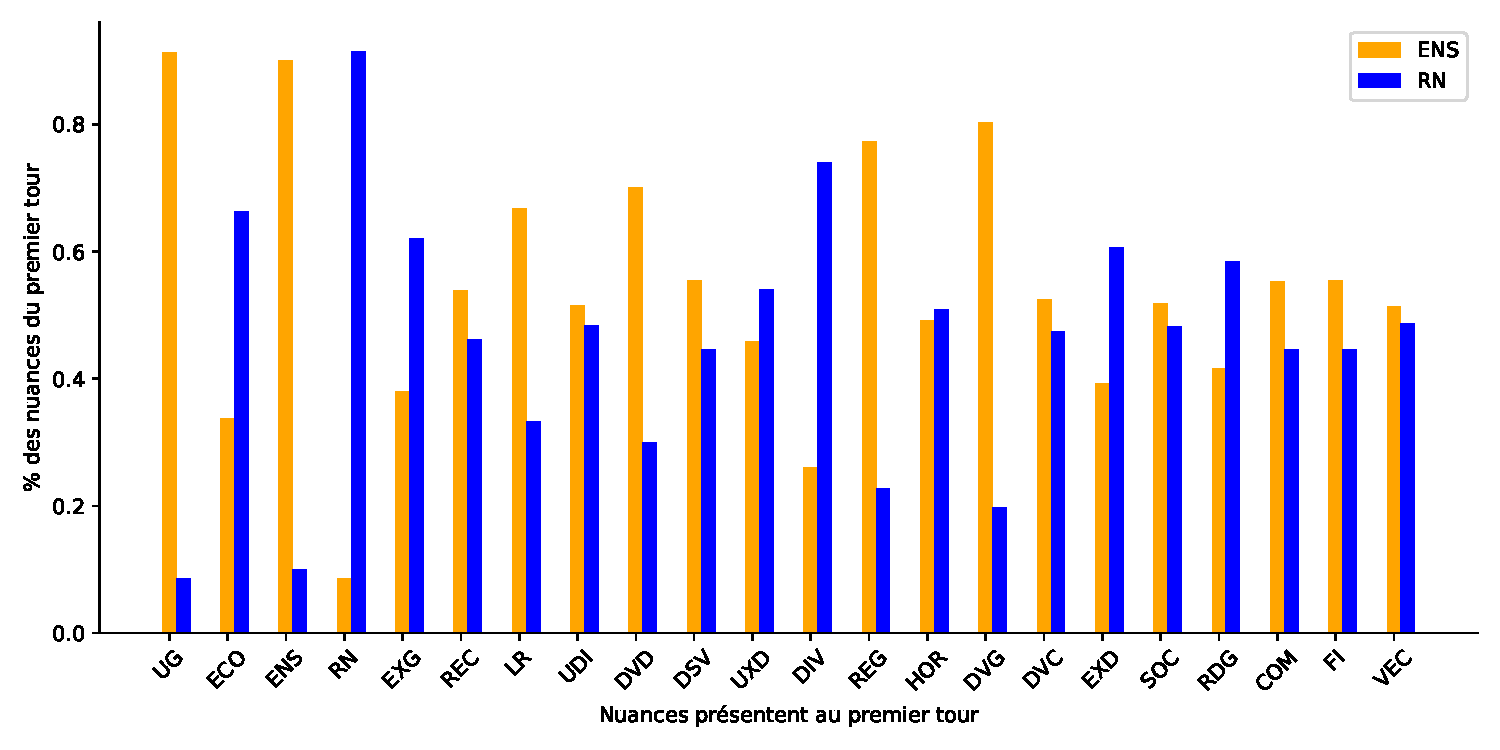
\includegraphics[width=0.7\textwidth]{Focus_ENS_RN.pdf}
                    \caption{Taux de report de chaque parti du premier tour vers l'un des deux candidat du second tour, lors des face-à-face entre ENS et le RN.}
                    \label{fig:ENS-RN}
                \end{center}
            \end{figure}
            \begin{figure}
                \begin{center}
                    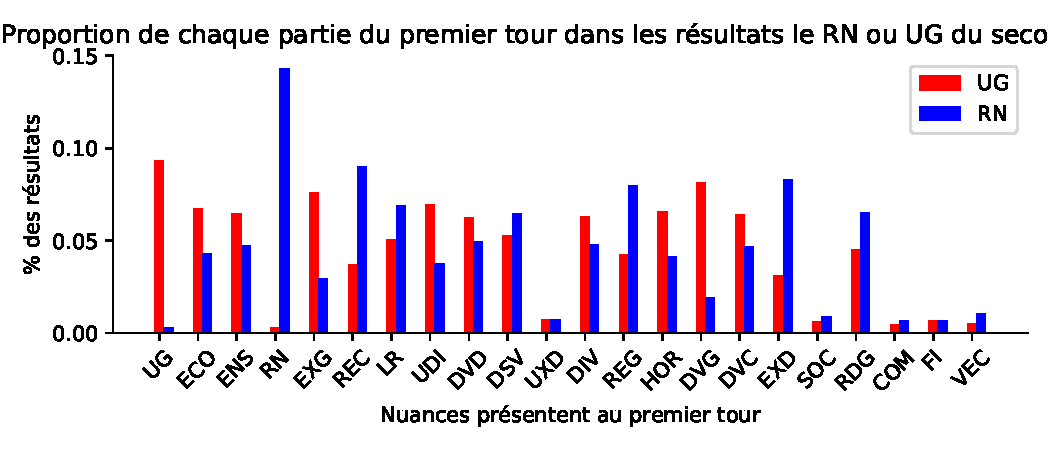
\includegraphics[width=0.7\textwidth]{Focus_UG_RN.pdf}
                    \caption{Taux de report de chaque parti du premier tour vers l'un des deux candidat du second tour, lors des face-à-face entre UG et le RN.}
                    \label{fig:UG-RN}
                \end{center}
            \end{figure}
            \begin{figure}
                \begin{center}
                    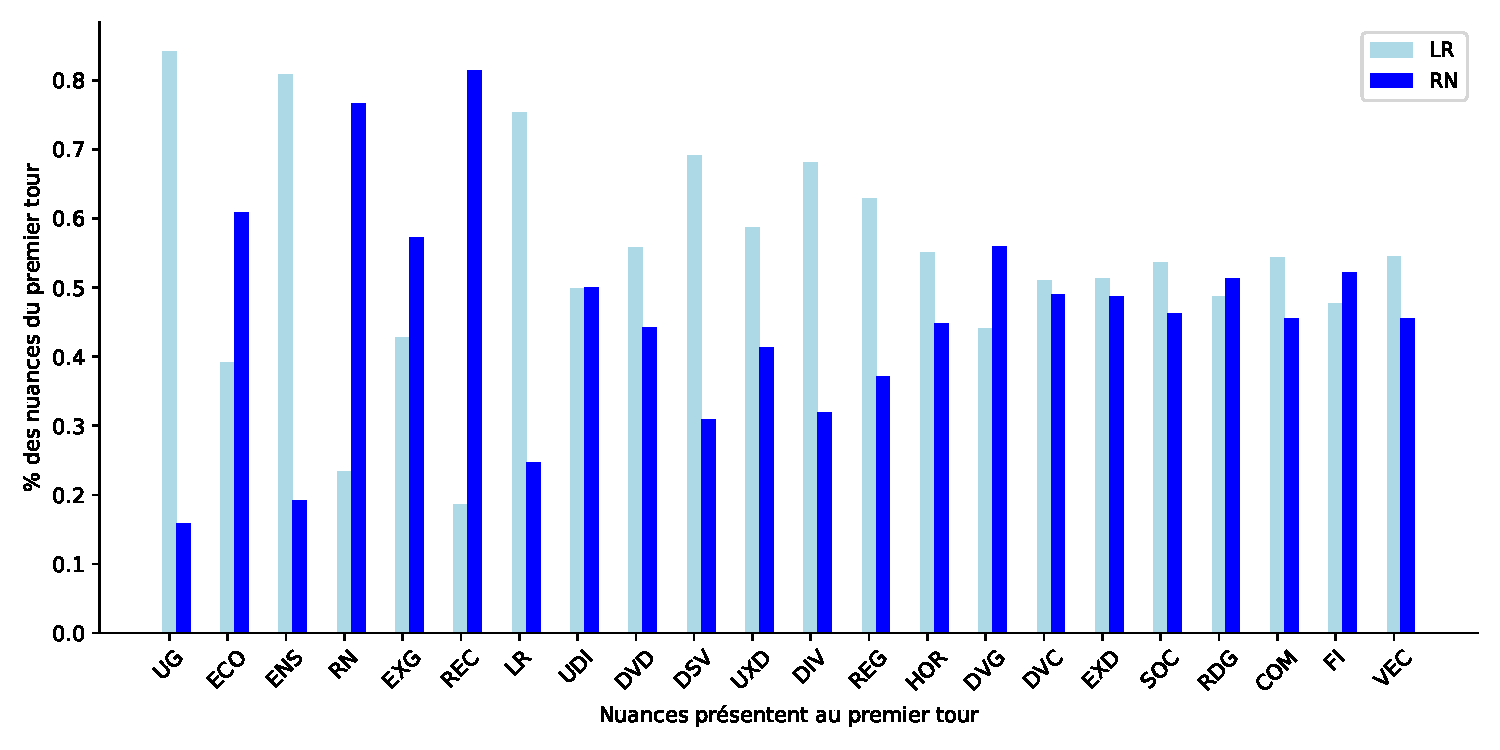
\includegraphics[width=0.7\textwidth]{Focus_LR_RN.pdf}
                    \caption{Taux de report de chaque parti du premier tour vers l'un des deux candidat du second tour, lors des face-à-face entre LR et le RN.}
                    \label{fig:LR-RN}
                \end{center}
            \end{figure}

        \subsection*{Généralisation nationale}
            
            Pour complexifier un peu plus la tâche, et enfin répondre au mieux à notre problématique, il a été possible de considérer le jeu de données dans son intégralité, et d'en extraire la matrice de transfert permettant de prédire au mieux les résultats du second tour. On remarque alors sur la partie gauche de la figure \ref{fig:True-Pred-Total} une zone large entourant la diagonale rouge. Bien qu'une plus grande densité soit présente autour de cette diagonale, on distingue nettement un second groupe dont les résultats sont sous-évalués par le modèle. Si l’on se penche sur l'extrapolation de la matrice de transfert de voix permettant de représenter les résultats de chaque nuance du second tour, sous la forme d'une somme des partis présents au premier tour, on remarque que la nuance la plus présente pour chaque parti est elle-même. Ce taux de A vers A est même majoritaire pour les plus petites nuances (LR, UXD, DVD, HOR, DVC, REG, etc.). Néanmoins, cela est moins vrai pour Ensemble et l'Union de la Gauche, présentant respectivement 46 \% et 32 \%, et encore moins pour le Rassemblement National avec seulement 21 \%. En se focalisant sur le RN, on remarque que ses voix viennent principalement de l'Extrême gauche et de Reconquête. Ce dernier est particulièrement présent chez UG et disparaît chez ENS.

            \begin{figure}[h]
                \begin{center}
                    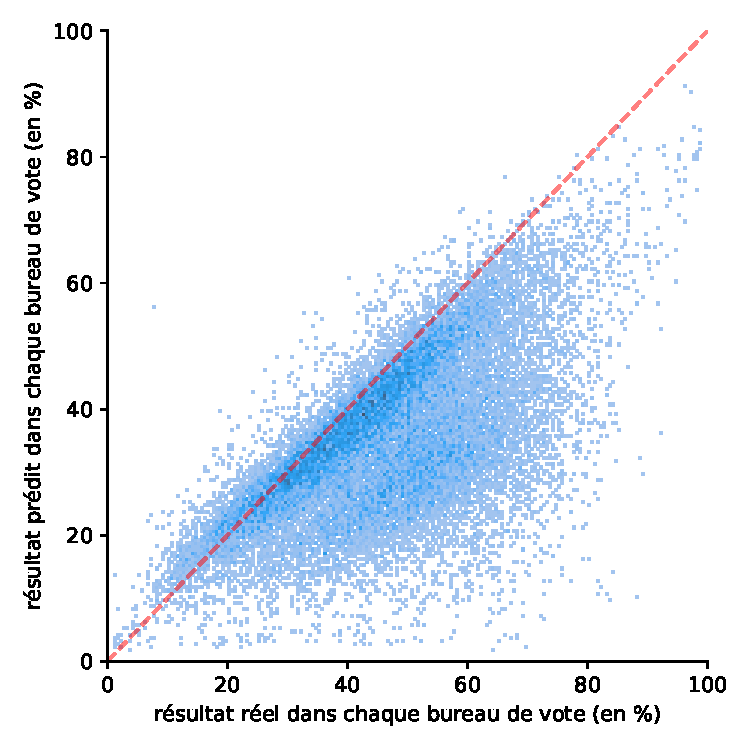
\includegraphics[height=5cm]{Total_True_Pred_Hist.pdf}
                    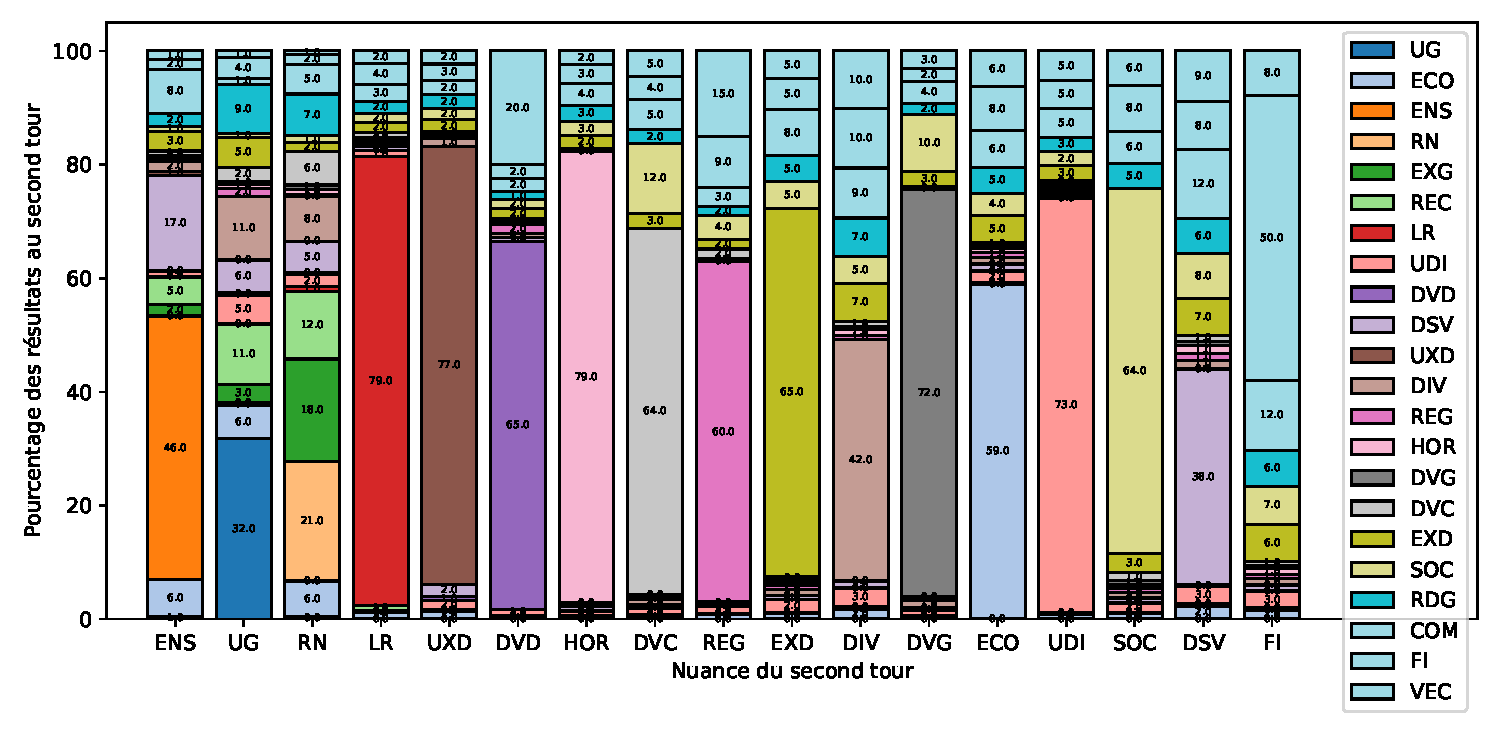
\includegraphics[height=5cm]{Total-Matrice-Participation.pdf}
                    \caption{Gauche) Représentation des résultats prédit pour chaque bureau de vote en fonction des résultats réels. Droite) Taux de représentation estimé de chaque nuance du premier tour dans les résultats de chaque nuance du second tour.}
                    \label{fig:True-Pred-Total}
                \end{center}
            \end{figure}
        
    \newpage
    %-------------------------
    % Discussion (1page) + Références
    %-------------------------
    \section{Discussion}
        Ce projet a eu pour objectif de développer une analyse visant à explorer les résultats des élections législatives anticipées de 2024 en France. Le principal objectif était donc de retrouver une matrice permettant de transformer la distribution des votes au premier tour en celle des votes au second.
        À un niveau très simplifié, le modèle fonctionne mais tend à surestimer ou sous-estimer les résultats, ce qui est probablement dû à une mauvaise répartition des nuances au sein des "familles", ainsi qu'aux différences dans le nombre de votes obtenus au total pour chacune.
        Lorsque l'on complexifie la tâche en considérant toutes les nuances mais en se concentrant uniquement sur des cas particuliers, on remarque que les prédictions sont bien meilleures, avec des mouvements plus logiques entre les "familles" politiques.
    
        Enfin, dans le cas le plus complexe, la précision semble bonne, mais on remarque une forte propension du modèle à sous-estimer une bonne partie des résultats. Un schéma récurrent est qu'une nuance arrivée en tête au premier tour remporte le second tour. Il est important de noter que, dans les cas où le Rassemblement National est arrivé en première position au premier tour, certains partis arrivés troisième, et pouvant participer au tour suivant, se sont désistés afin de permettre au deuxième de dépasser le RN lors du second tour. Ce "front républicain" va par conséquent à l'encontre du schéma récurrent présenté plus haut et pourrait expliquer une sous-estimation du modèle qui ne prend pas cet élément en considération.

        Cette méthode permet donc d'estimer une matrice de transition pouvant être assimilée à un report des voix, mais semble quelque peu limitée dans ce contexte par le nombre possible de face-à-face. De plus, il n'est raisonnablement pas possible de trouver le taux réel de report entre deux nuances en se basant uniquement sur les résultats, car celui-ci dépend probablement de paramètres géographiques et socio-économiques. Ensuite, ce taux de report généralise une règle pour l'ensemble d'une nuance et passe donc au-dessus des possibles divergences présentes. Un exemple particulièrement frappant, mais ne rentrant pas en jeu ici, est le cas des Républicain et de la discorde entre sa présidence et certains de ses adhérents.

    \printbibliography

\end{document}